\documentclass{article}

\usepackage{graphicx}
\usepackage{float}
\usepackage{geometry}
\usepackage{listings}
\usepackage{subcaption}
\usepackage{amsmath}

\geometry{margin=1in}

\title{EEE3307: Experiment \#1}
\author{Yousef Alaa Awad, Abram Tadros, and Egor Shevchenko}
\date{\today}

\begin{document}

\maketitle
\tableofcontents
\newpage

%%%%%%%%%%%%%%%%%%%%%%%%%%%%%%%%%%%%%%%%%%%%%%%%%%%%%%%%%%%%%%%%%%%%%%%%%%%%%%%%%%%%%%%%
\section{Objective}
The primary objective of this experiment was to familiarize the laboratory group with the interplay between software simulation (LTSpice) and physical laboratory instrumentation. Specifically, the experiment aimed to:
\begin{enumerate}
    \item Analyze the transient response of a diode half-wave rectifier circuit.
    \item Analyze the DC operating point characteristics of a diode-resistor circuit.
    \item Verify theoretical models and simulations against physical measurements taken with a Tektronix oscilloscope and digital multimeter.
\end{enumerate}

%%%%%%%%%%%%%%%%%%%%%%%%%%%%%%%%%%%%%%%%%%%%%%%%%%%%%%%%%%%%%%%%%%%%%%%%%%%%%%%%%%%%%%%%
\section{Procedure}

\subsection{Part 1: AC Transient Analysis (Half-Wave Rectifier)}
A series circuit consisting of a sinusoidal voltage source, a 1N4148 diode, and a $1\text{k}\Omega$ resistor was constructed.
\begin{itemize}
    \item \textbf{Simulation:} The circuit was simulated in LTSpice using a sinusoidal input with an amplitude of 4V (8V peak-to-peak) at 5kHz. The output voltage across the resistor was plotted.
    \item \textbf{Experiment:} The physical circuit was built on a breadboard. A function generator was configured to produce the same 4V amplitude, 5kHz sine wave. The output waveform was captured using a Tektronix oscilloscope.
\end{itemize}

\subsection{Part 2: DC Operating Point Analysis}
A DC voltage source was placed in series with the diode and the $1\text{k}\Omega$ resistor.
\begin{itemize}
    \item \textbf{Simulation:} An operating point (\texttt{.op}) simulation was run for input voltages ($V_B$) of 1V and 2V to determine the expected loop current.
    \item \textbf{Experiment:} The DC power supply was set to 1V and subsequently 2V. The current flowing through the circuit was measured using a digital multimeter (DMM).
\end{itemize}

\pagebreak
%%%%%%%%%%%%%%%%%%%%%%%%%%%%%%%%%%%%%%%%%%%%%%%%%%%%%%%%%%%%%%%%%%%%%%%%%%%%%%%%%%%%%%%%
\section{Simulation Results}

\subsection{AC Simulation}
The LTSpice simulation for the AC transient analysis is shown below. The input source was defined as \texttt{SINE(0 4 5k)}. The output waveform demonstrates half-wave rectification, where the negative cycle is clipped, and the positive peak is reduced by the diode forward voltage drop ($\approx 0.7\text{V}$).

\begin{figure}[!ht]
    \centering
    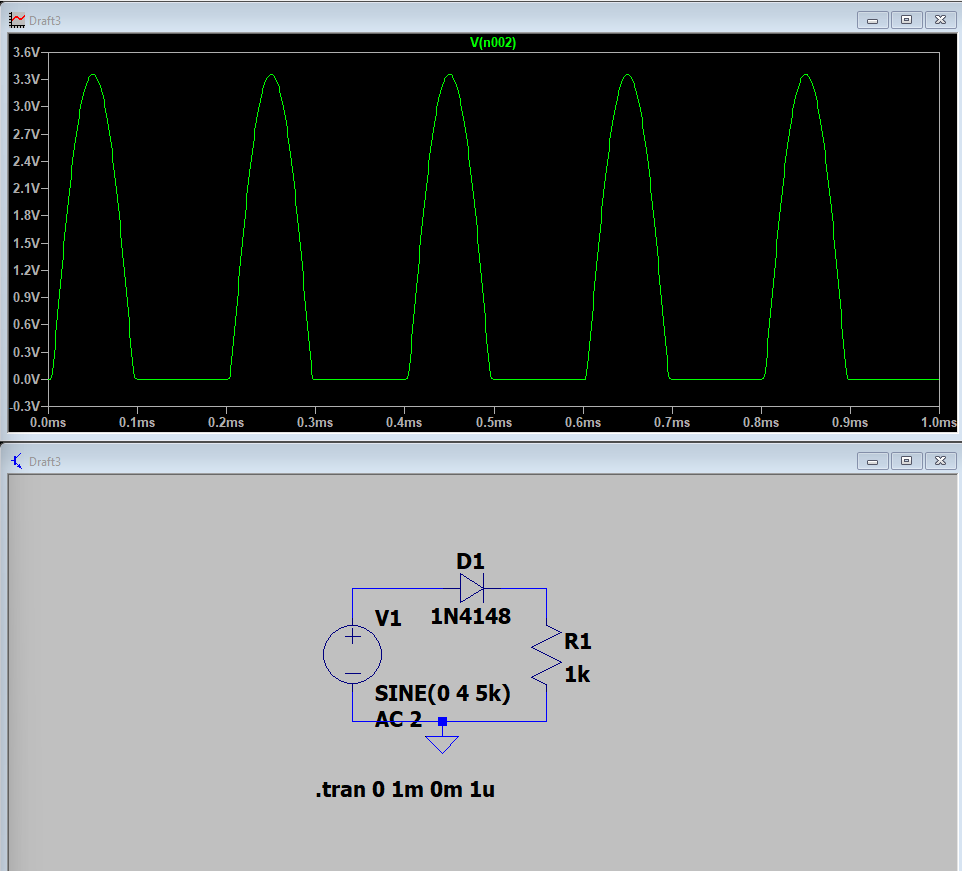
\includegraphics[width=0.8\textwidth]{Pictures/simulation_waveform.png}
    \caption{LTSpice simulation of the half-wave rectifier output. The peak output voltage is approximately 3.3V.}
    \label{fig:sim_wave}
\end{figure}

\subsection{DC Simulation}
The operating point simulations provided the theoretical current values for the DC analysis.
\begin{itemize}
    \item At $V_{in} = 1\text{V}$, the calculated current was $0.370\text{mA}$.
    \item At $V_{in} = 2\text{V}$, the calculated current was $1.337\text{mA}$.
\end{itemize}

\begin{figure}[!ht]
    \centering
    \begin{subfigure}[b]{0.48\textwidth}
        \centering
        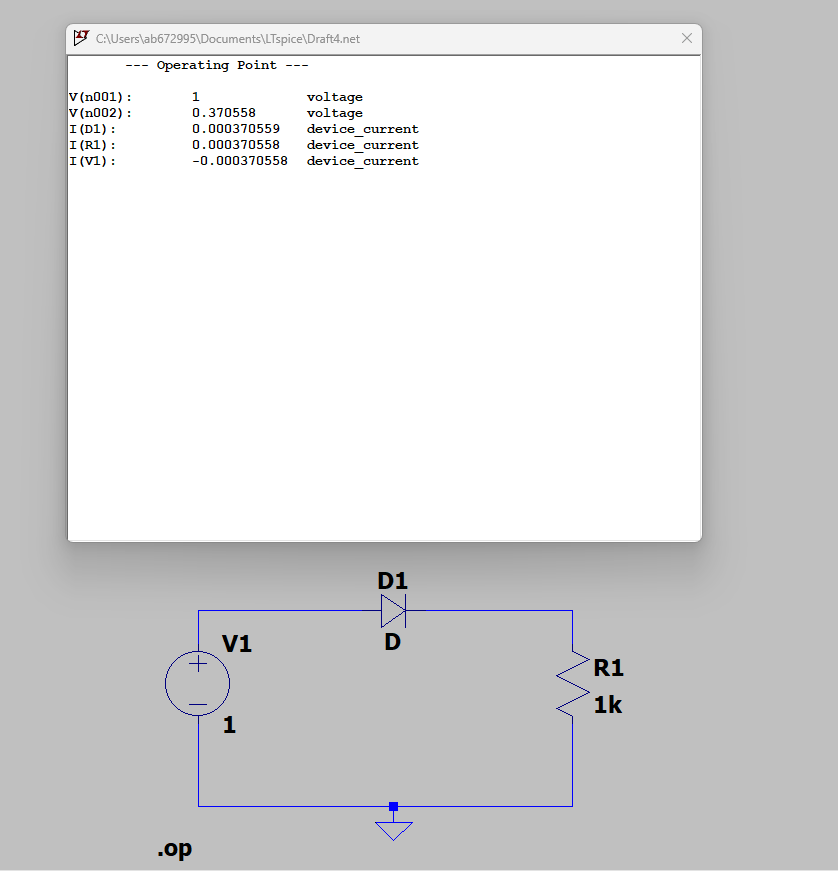
\includegraphics[width=\textwidth]{Pictures/simulation_numbers_1v.png}
        \caption{Simulation at 1V input.}
        \label{fig:sim_1v}
    \end{subfigure}
    \hfill
    \begin{subfigure}[b]{0.48\textwidth}
        \centering
        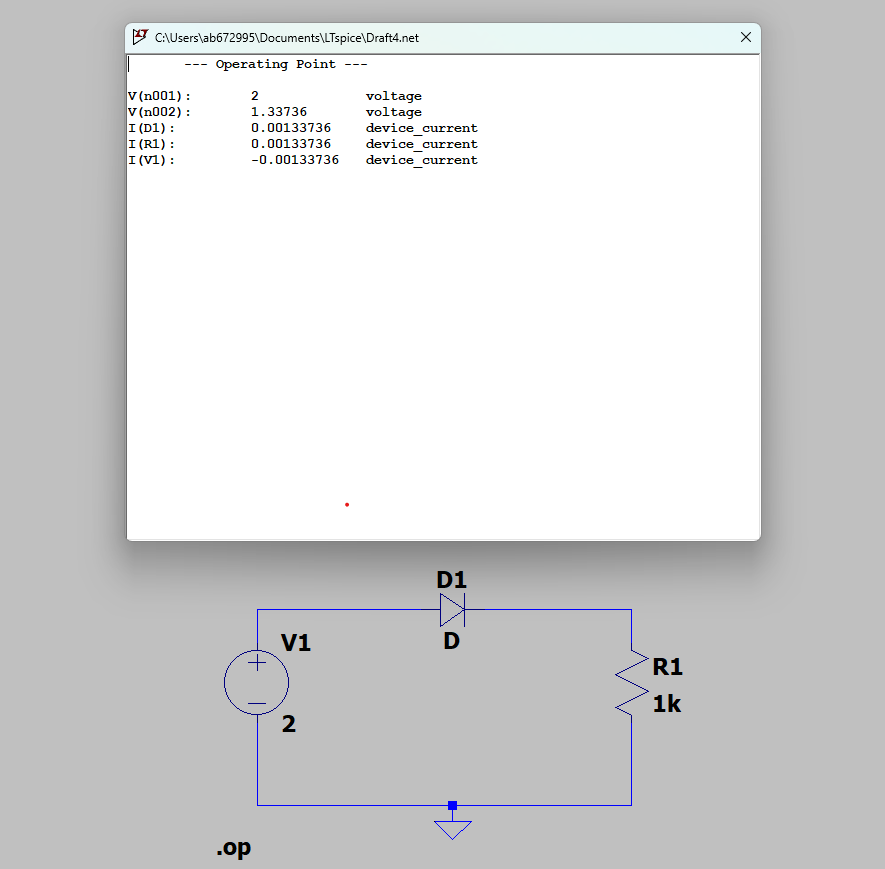
\includegraphics[width=\textwidth]{Pictures/simulation_numbers_2v.png}
        \caption{Simulation at 2V input.}
        \label{fig:sim_2v}
    \end{subfigure}
    \caption{LTSpice Operating Point results showing device current.}
\end{figure}

\pagebreak
%%%%%%%%%%%%%%%%%%%%%%%%%%%%%%%%%%%%%%%%%%%%%%%%%%%%%%%%%%%%%%%%%%%%%%%%%%%%%%%%%%%%%%%%
\section{Experimental Results}

\subsection{AC Measurement}
The oscilloscope capture of the physical circuit is shown in Figure \ref{fig:exp_wave}. The waveform matches the simulation characteristic, showing a clear rectified sine wave. The measured peak-to-peak voltage (which effectively represents the positive peak amplitude in this rectified signal) was $3.35\text{V}$.

\begin{figure}[!ht]
    \centering
    \includegraphics[width=0.7\textwidth]{Pictures/waveform_actual.jpeg}
    \caption{Oscilloscope capture of the output voltage across the resistor. Measured Vpp is 3.351V.}
    \label{fig:exp_wave}
\end{figure}

\subsection{DC Measurement}
The current was measured using the DMM for both voltage cases.
\begin{itemize}
    \item At $V_{in} = 1\text{V}$, the measured current was $0.4176\text{mA}$.
    \item At $V_{in} = 2\text{V}$, the measured current was $1.3603\text{mA}$.
\end{itemize}

\begin{figure}[!ht]
    \centering
    \begin{subfigure}[b]{0.48\textwidth}
        \centering
        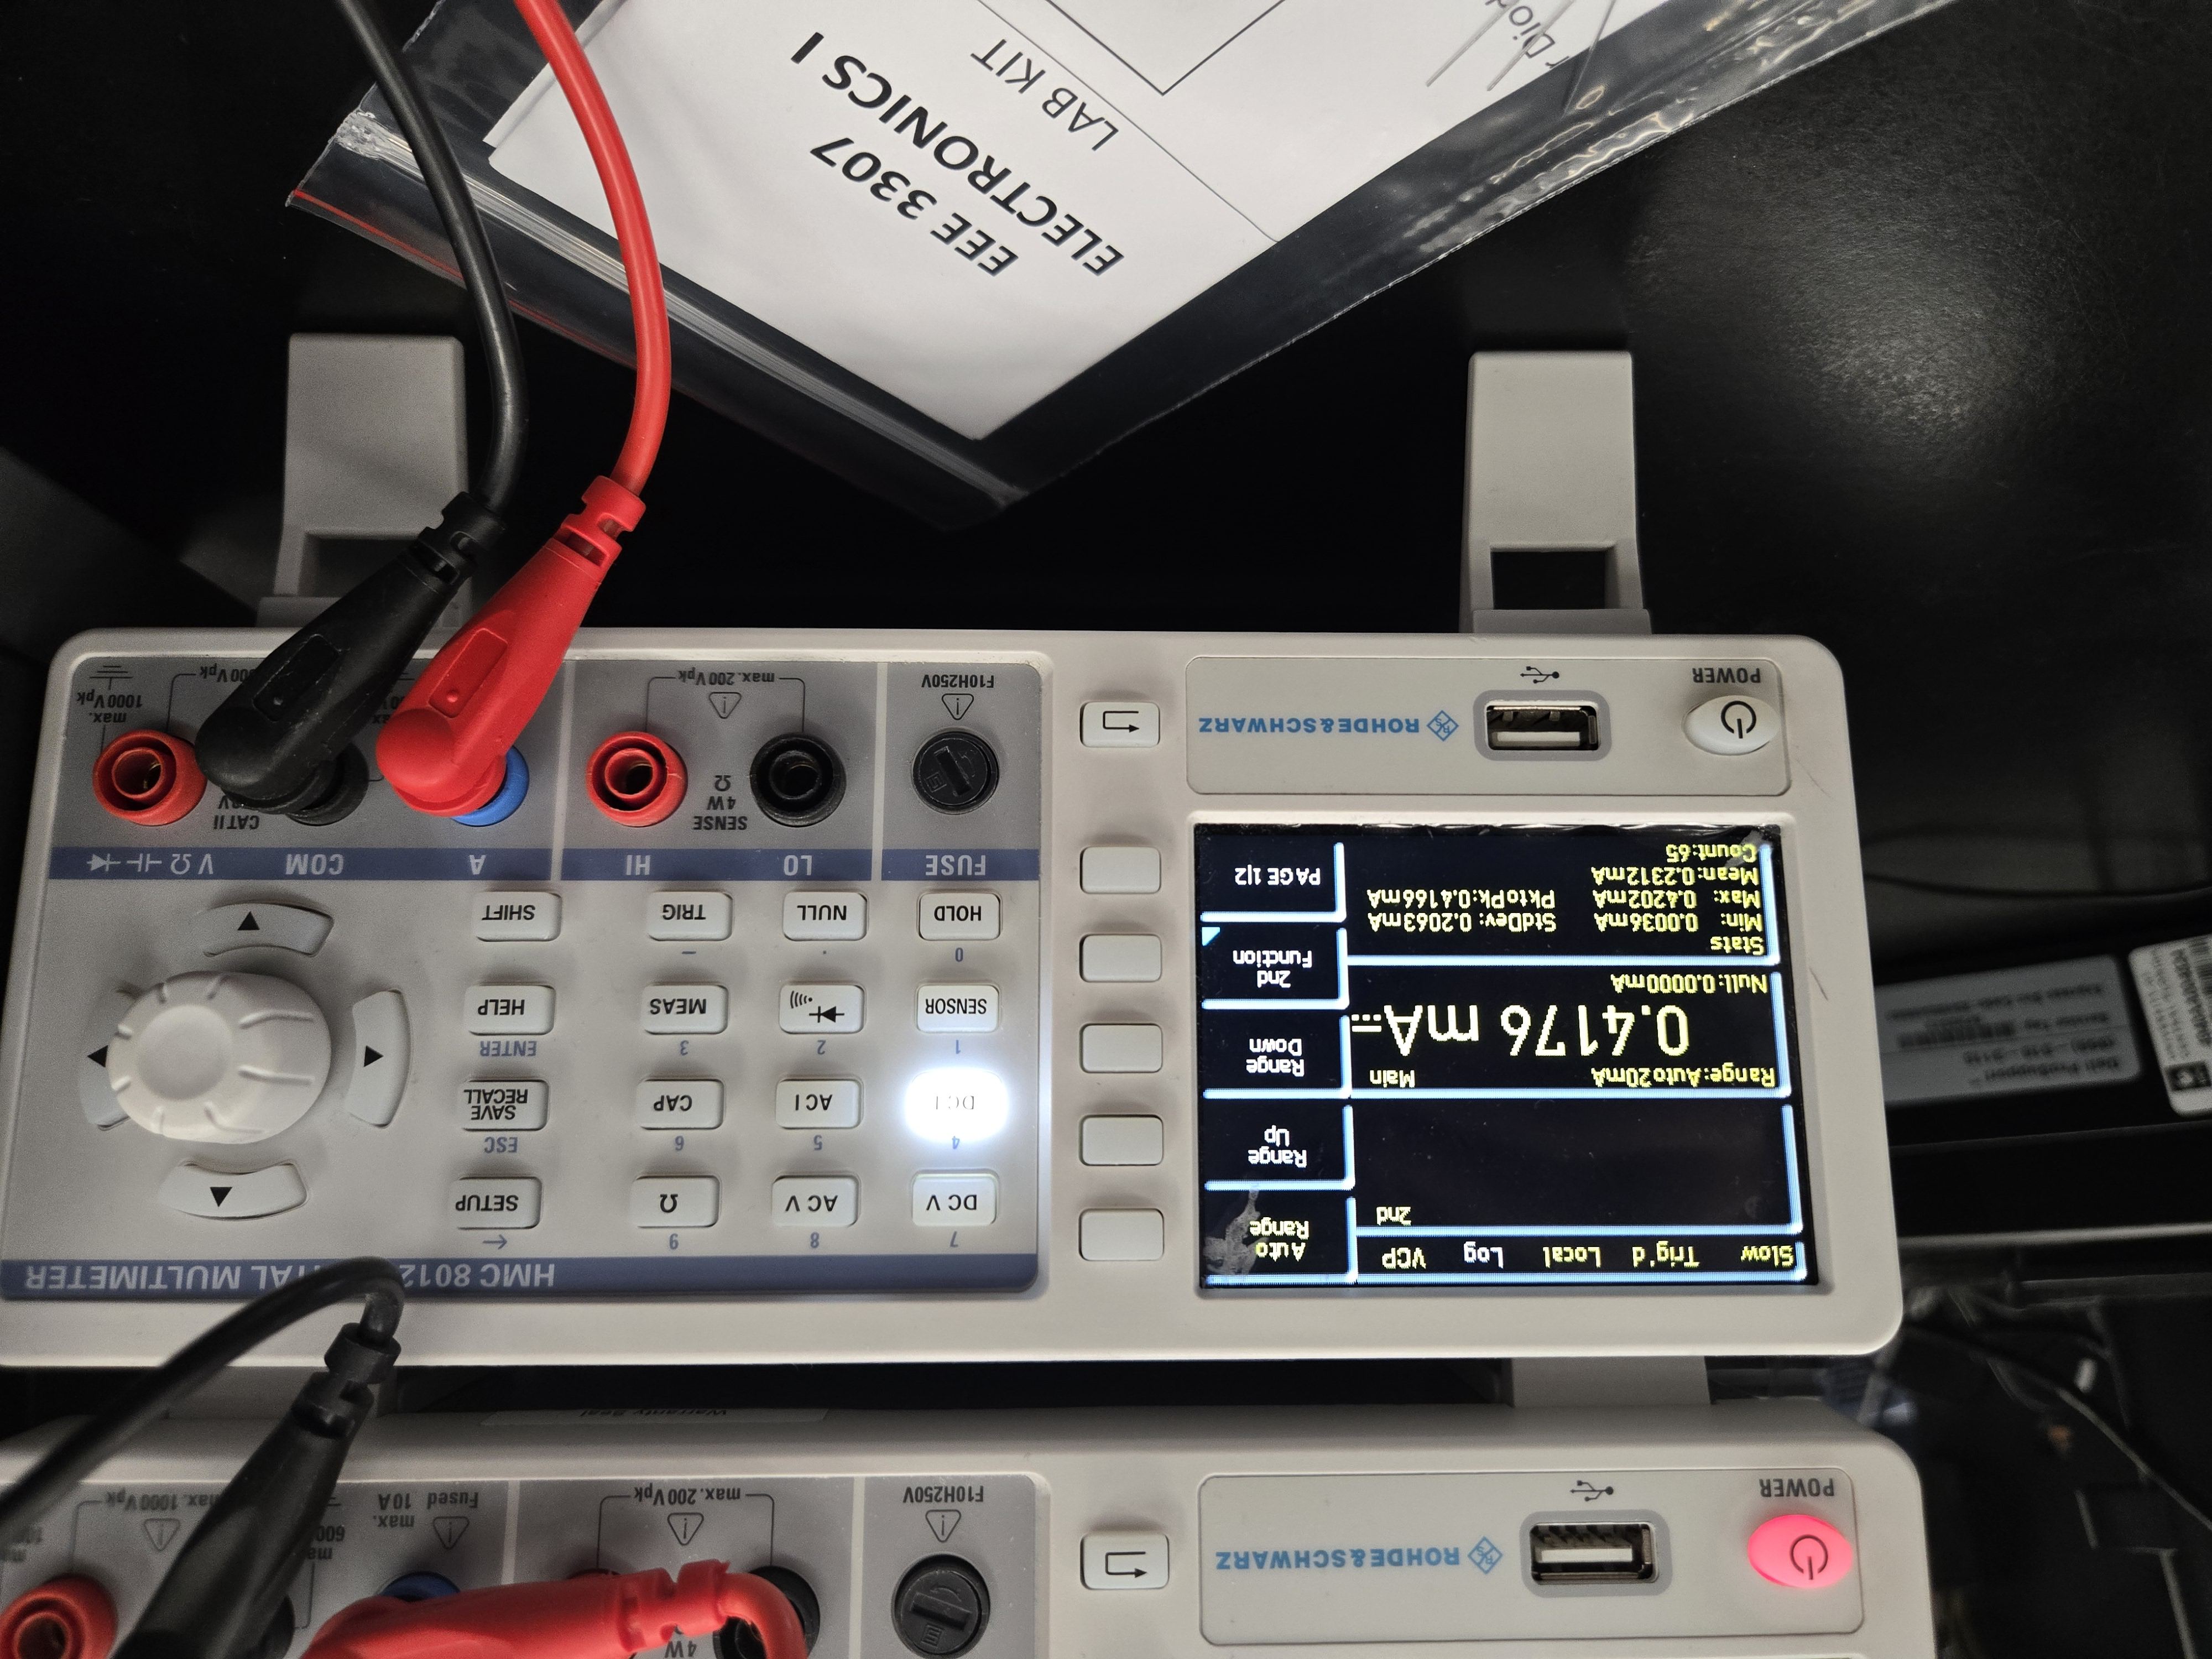
\includegraphics[width=\textwidth, angle=-180]{Pictures/measured_amperage_1v.jpg}
        \caption{Measured current at 1V input: 0.4176 mA.}
        \label{fig:meas_1v}
    \end{subfigure}
    \hfill
    \begin{subfigure}[b]{0.48\textwidth}
        \centering
        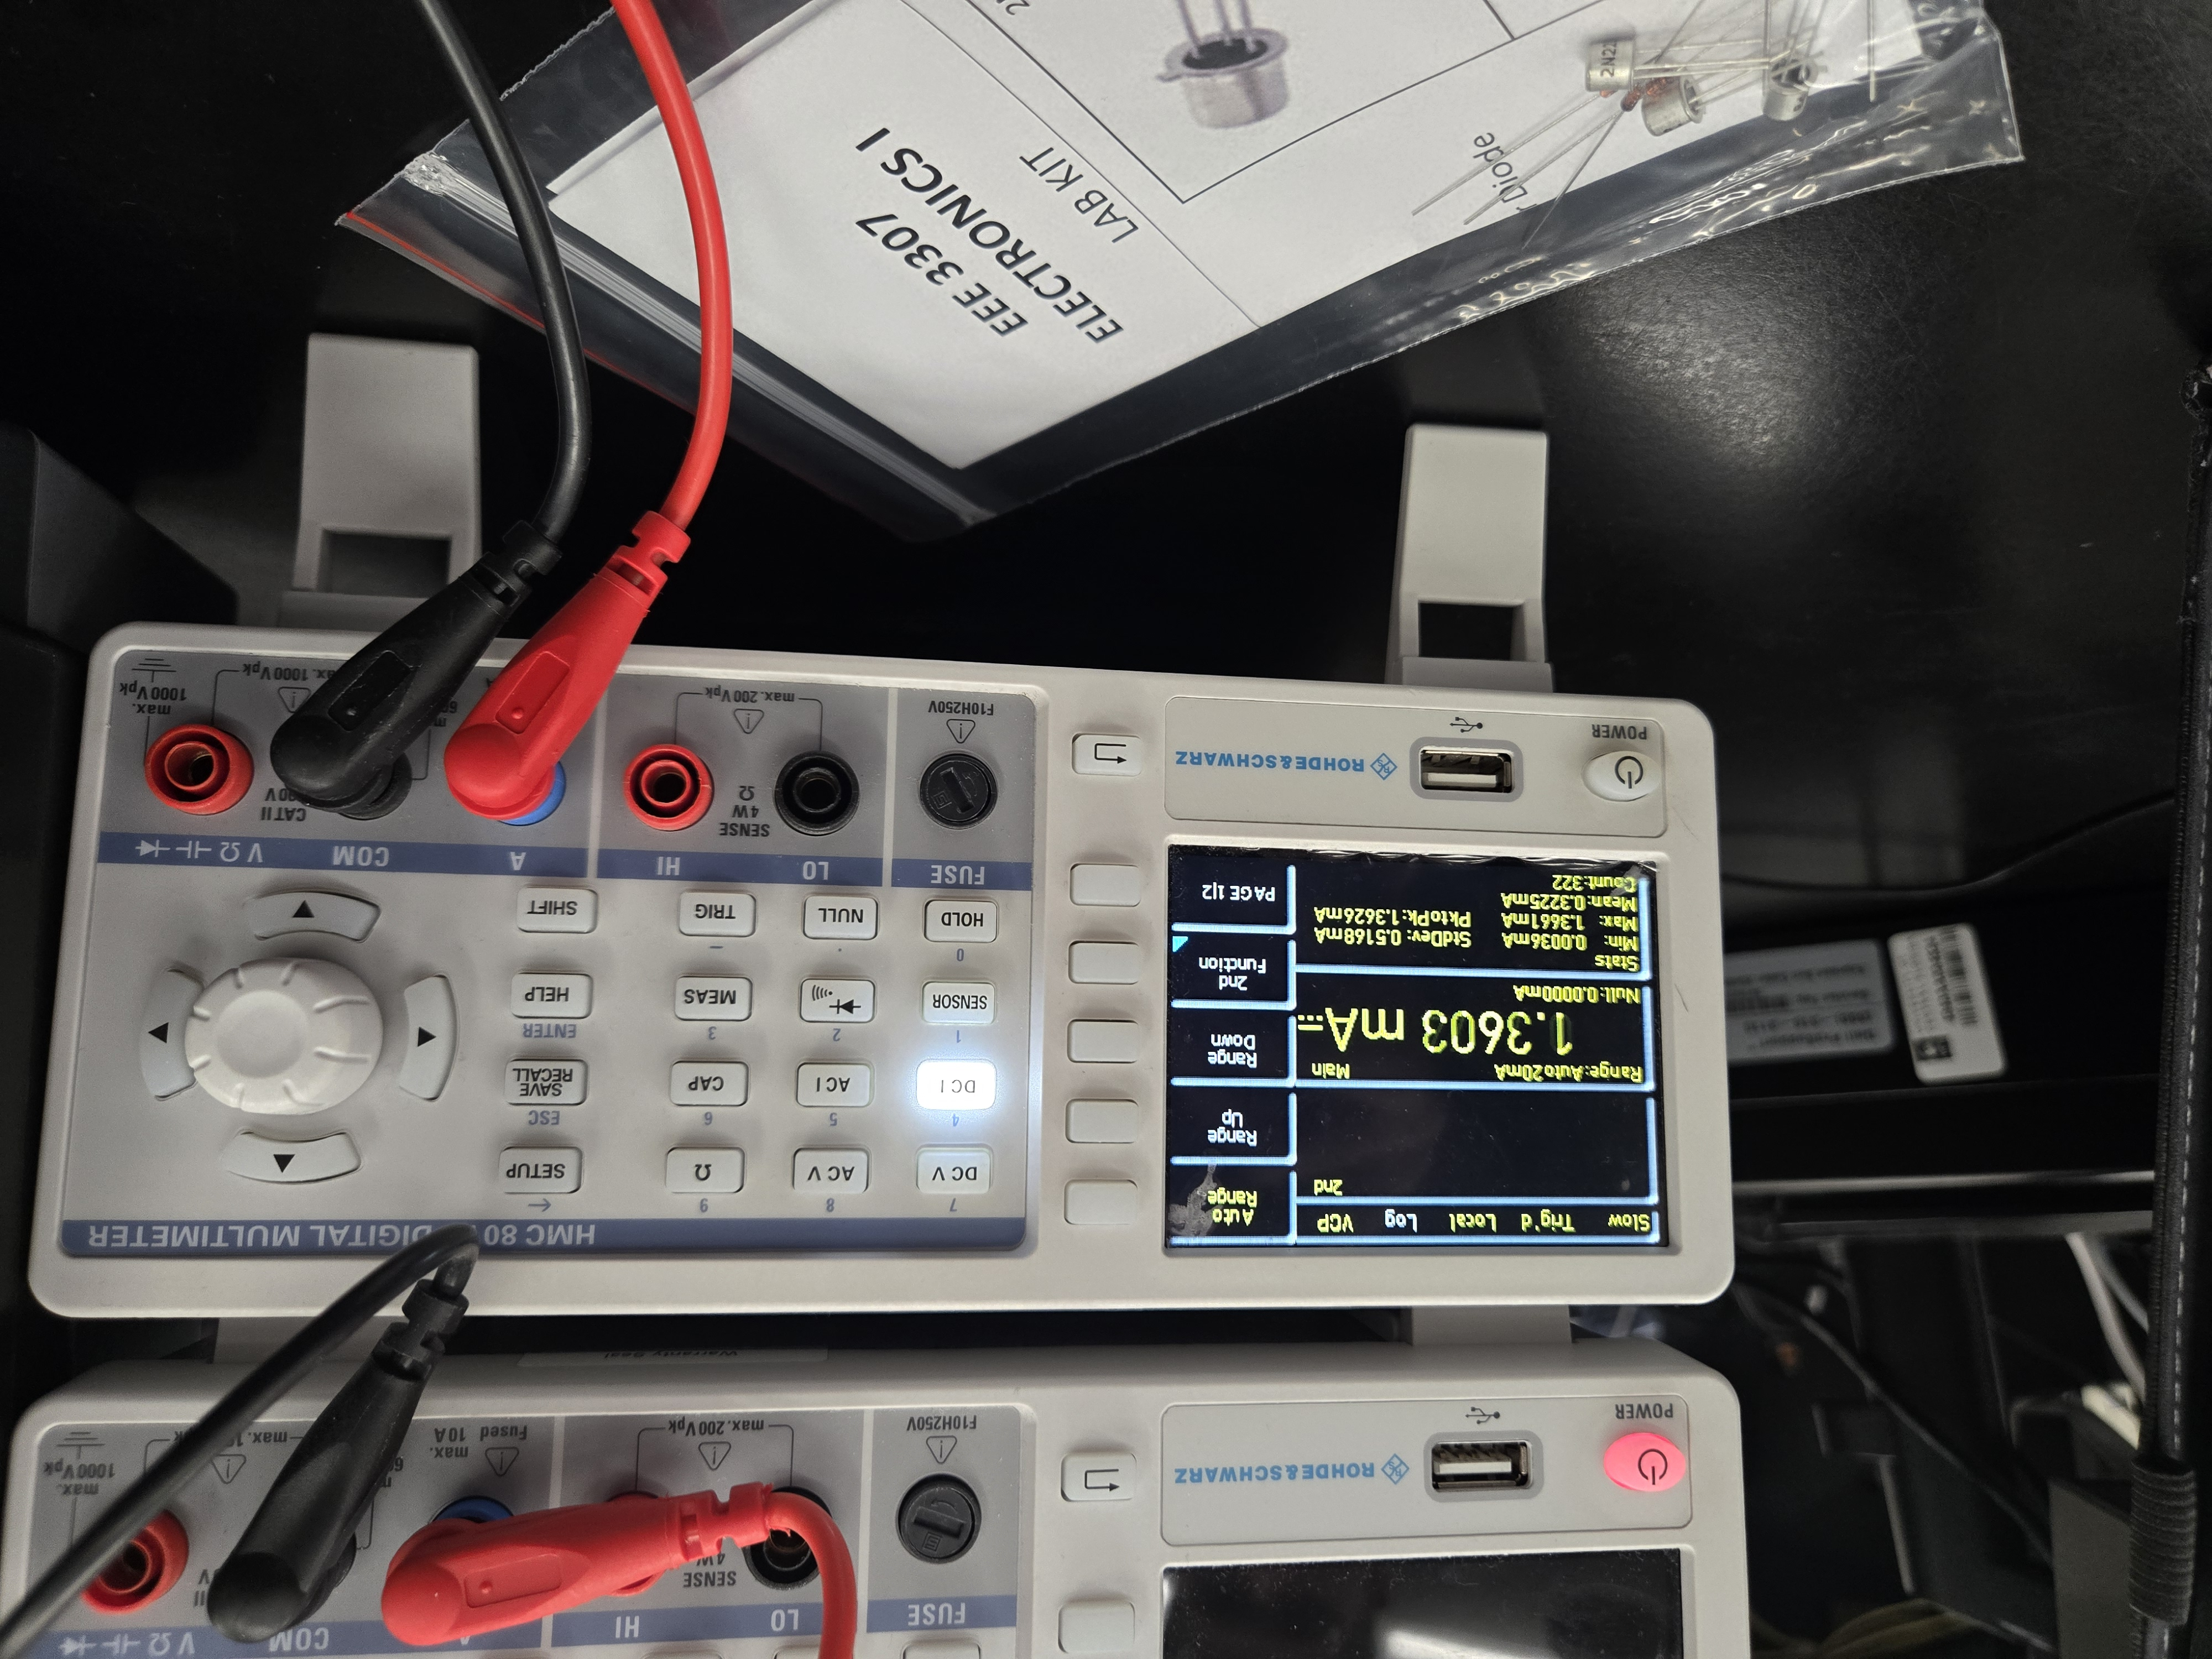
\includegraphics[width=\textwidth, angle=-180]{Pictures/measured_amperage_2v.jpg}
        \caption{Measured current at 2V input: 1.3603 mA.}
        \label{fig:meas_2v}
    \end{subfigure}
    \caption{Digital Multimeter current readings.}
\end{figure}

\pagebreak
%%%%%%%%%%%%%%%%%%%%%%%%%%%%%%%%%%%%%%%%%%%%%%%%%%%%%%%%%%%%%%%%%%%%%%%%%%%%%%%%%%%%%%%%
\section{Discussion and Error Analysis}

\subsection{AC Analysis Comparison}
Both the simulation and the experimental results showed a peak output voltage of approximately $3.3\text{V}$ given a $4\text{V}$ peak input.
\begin{itemize}
    \item \textbf{Simulation Peak:} $\approx 3.3\text{V}$
    \item \textbf{Experimental Peak:} $3.35\text{V}$
\end{itemize}
The voltage drop across the diode is consistent with the theoretical silicon diode drop: $4\text{V} - 3.35\text{V} \approx 0.65\text{V}$. The experimental result is extremely close to the simulation, validating the transient model of the diode.

\subsection{DC Analysis Comparison}
Table \ref{tab:dc_comparison} summarizes the difference between the simulated and measured currents.

\begin{table}[!ht]
    \centering
    \begin{tabular}{|c|c|c|c|}
        \hline
        \textbf{Input Voltage (V)} & \textbf{Simulated Current (mA)} & \textbf{Measured Current (mA)} & \textbf{\% Difference} \\
        \hline
        1V & 0.370 & 0.4176 & 12.8\% \\
        \hline
        2V & 1.337 & 1.3603 & 1.7\% \\
        \hline
    \end{tabular}
    \caption{Comparison of DC Current values.}
    \label{tab:dc_comparison}
\end{table}

The error at 2V is negligible ($1.7\%$). The higher relative error at 1V ($12.8\%$) is likely due to the non-linear nature of the diode. At 1V, the diode is operating closer to its "minimum" voltage. Small variations between the idealized SPICE model (1N4148) and the physical diode's specific IV curve, or slight deviations in the actual resistor value (tolerance), have a more significant impact on the current at lower voltages. However, the general behavior is consistent.

%%%%%%%%%%%%%%%%%%%%%%%%%%%%%%%%%%%%%%%%%%%%%%%%%%%%%%%%%%%%%%%%%%%%%%%%%%%%%%%%%%%%%%%%
\section{Conclusion}
This experiment successfully demonstrated the operation of a diode as a non-linear circuit element. The half-wave rectifier circuit behaved as predicted, passing only the positive half of the AC signal minus the diode forward voltage drop. The DC measurements confirmed the diode's biasing characteristics, with experimental data aligning closely with LTSpice simulations, particularly at higher bias voltages. The slight discrepancies observed are attributable to real-world component tolerances and model variations, which are expected in a laboratory setting.

\end{document}
